% Created by tikzDevice version 0.12.3.1 on 2021-11-23 19:17:22
% !TEX encoding = UTF-8 Unicode
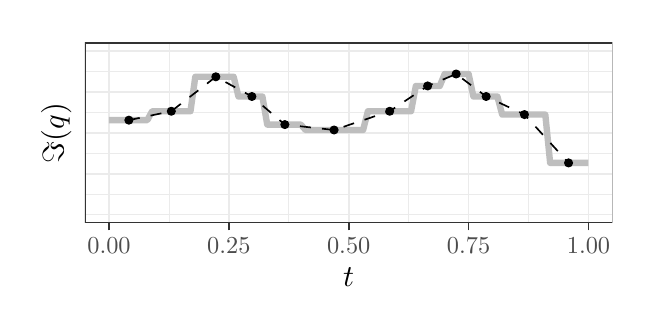
\begin{tikzpicture}[x=1pt,y=1pt]
\definecolor{fillColor}{RGB}{255,255,255}
\path[use as bounding box,fill=fillColor,fill opacity=0.00] (0,0) rectangle (216.81,101.18);
\begin{scope}
\path[clip] (  0.00,  0.00) rectangle (216.81,101.18);
\definecolor{drawColor}{RGB}{255,255,255}
\definecolor{fillColor}{RGB}{255,255,255}

\path[draw=drawColor,line width= 0.6pt,line join=round,line cap=round,fill=fillColor] (  0.00,  0.00) rectangle (216.81,101.18);
\end{scope}
\begin{scope}
\path[clip] ( 20.71, 30.69) rectangle (211.31, 95.68);
\definecolor{fillColor}{RGB}{255,255,255}

\path[fill=fillColor] ( 20.71, 30.69) rectangle (211.31, 95.68);
\definecolor{drawColor}{gray}{0.92}

\path[draw=drawColor,line width= 0.3pt,line join=round] ( 20.71, 41.03) --
	(211.31, 41.03);

\path[draw=drawColor,line width= 0.3pt,line join=round] ( 20.71, 55.80) --
	(211.31, 55.80);

\path[draw=drawColor,line width= 0.3pt,line join=round] ( 20.71, 70.57) --
	(211.31, 70.57);

\path[draw=drawColor,line width= 0.3pt,line join=round] ( 20.71, 85.34) --
	(211.31, 85.34);

\path[draw=drawColor,line width= 0.3pt,line join=round] ( 51.04, 30.69) --
	( 51.04, 95.68);

\path[draw=drawColor,line width= 0.3pt,line join=round] ( 94.35, 30.69) --
	( 94.35, 95.68);

\path[draw=drawColor,line width= 0.3pt,line join=round] (137.67, 30.69) --
	(137.67, 95.68);

\path[draw=drawColor,line width= 0.3pt,line join=round] (180.99, 30.69) --
	(180.99, 95.68);

\path[draw=drawColor,line width= 0.6pt,line join=round] ( 20.71, 33.64) --
	(211.31, 33.64);

\path[draw=drawColor,line width= 0.6pt,line join=round] ( 20.71, 48.41) --
	(211.31, 48.41);

\path[draw=drawColor,line width= 0.6pt,line join=round] ( 20.71, 63.18) --
	(211.31, 63.18);

\path[draw=drawColor,line width= 0.6pt,line join=round] ( 20.71, 77.95) --
	(211.31, 77.95);

\path[draw=drawColor,line width= 0.6pt,line join=round] ( 20.71, 92.72) --
	(211.31, 92.72);

\path[draw=drawColor,line width= 0.6pt,line join=round] ( 29.38, 30.69) --
	( 29.38, 95.68);

\path[draw=drawColor,line width= 0.6pt,line join=round] ( 72.69, 30.69) --
	( 72.69, 95.68);

\path[draw=drawColor,line width= 0.6pt,line join=round] (116.01, 30.69) --
	(116.01, 95.68);

\path[draw=drawColor,line width= 0.6pt,line join=round] (159.33, 30.69) --
	(159.33, 95.68);

\path[draw=drawColor,line width= 0.6pt,line join=round] (202.65, 30.69) --
	(202.65, 95.68);
\definecolor{drawColor}{RGB}{190,190,190}

\path[draw=drawColor,line width= 2.3pt,line join=round] ( 29.38, 67.76) --
	( 31.11, 67.76) --
	( 32.84, 67.76) --
	( 34.58, 67.76) --
	( 36.31, 67.76) --
	( 38.04, 67.76) --
	( 39.77, 67.76) --
	( 41.51, 67.76) --
	( 43.24, 67.76) --
	( 44.97, 70.98) --
	( 46.70, 70.98) --
	( 48.44, 70.98) --
	( 50.17, 70.98) --
	( 51.90, 70.98) --
	( 53.64, 70.98) --
	( 55.37, 70.98) --
	( 57.10, 70.98) --
	( 58.83, 70.98) --
	( 60.57, 83.43) --
	( 62.30, 83.43) --
	( 64.03, 83.43) --
	( 65.76, 83.43) --
	( 67.50, 83.43) --
	( 69.23, 83.43) --
	( 70.96, 83.43) --
	( 72.69, 83.43) --
	( 74.43, 83.43) --
	( 76.16, 76.31) --
	( 77.89, 76.31) --
	( 79.63, 76.31) --
	( 81.36, 76.31) --
	( 83.09, 76.31) --
	( 84.82, 76.31) --
	( 86.56, 66.16) --
	( 88.29, 66.16) --
	( 90.02, 66.16) --
	( 91.75, 66.16) --
	( 93.49, 66.16) --
	( 95.22, 66.16) --
	( 96.95, 66.16) --
	( 98.69, 66.16) --
	(100.42, 64.21) --
	(102.15, 64.21) --
	(103.88, 64.21) --
	(105.62, 64.21) --
	(107.35, 64.21) --
	(109.08, 64.21) --
	(110.81, 64.21) --
	(112.55, 64.21) --
	(114.28, 64.21) --
	(116.01, 64.21) --
	(117.74, 64.21) --
	(119.48, 64.21) --
	(121.21, 64.21) --
	(122.94, 70.98) --
	(124.68, 70.98) --
	(126.41, 70.98) --
	(128.14, 70.98) --
	(129.87, 70.98) --
	(131.61, 70.98) --
	(133.34, 70.98) --
	(135.07, 70.98) --
	(136.80, 70.98) --
	(138.54, 70.98) --
	(140.27, 80.12) --
	(142.00, 80.12) --
	(143.74, 80.12) --
	(145.47, 80.12) --
	(147.20, 80.12) --
	(148.93, 80.12) --
	(150.67, 84.44) --
	(152.40, 84.44) --
	(154.13, 84.44) --
	(155.86, 84.44) --
	(157.60, 84.44) --
	(159.33, 84.44) --
	(161.06, 76.31) --
	(162.79, 76.31) --
	(164.53, 76.31) --
	(166.26, 76.31) --
	(167.99, 76.31) --
	(169.73, 76.31) --
	(171.46, 69.78) --
	(173.19, 69.78) --
	(174.92, 69.78) --
	(176.66, 69.78) --
	(178.39, 69.78) --
	(180.12, 69.78) --
	(181.85, 69.78) --
	(183.59, 69.78) --
	(185.32, 69.78) --
	(187.05, 69.78) --
	(188.79, 52.31) --
	(190.52, 52.31) --
	(192.25, 52.31) --
	(193.98, 52.31) --
	(195.72, 52.31) --
	(197.45, 52.31) --
	(199.18, 52.31) --
	(200.91, 52.31) --
	(202.65, 52.31);
\definecolor{drawColor}{RGB}{0,0,0}

\path[draw=drawColor,line width= 0.6pt,dash pattern=on 4pt off 4pt ,line join=round] ( 36.57, 67.76) --
	( 51.90, 70.98) --
	( 67.99, 83.43) --
	( 81.02, 76.31) --
	( 92.93, 66.16) --
	(110.71, 64.21) --
	(130.82, 70.98) --
	(144.53, 80.12) --
	(154.83, 84.44) --
	(165.67, 76.31) --
	(179.51, 69.78) --
	(195.45, 52.31);
\definecolor{fillColor}{RGB}{0,0,0}

\path[draw=drawColor,line width= 0.4pt,line join=round,line cap=round,fill=fillColor] ( 36.57, 67.76) circle (  1.43);

\path[draw=drawColor,line width= 0.4pt,line join=round,line cap=round,fill=fillColor] ( 51.90, 70.98) circle (  1.43);

\path[draw=drawColor,line width= 0.4pt,line join=round,line cap=round,fill=fillColor] ( 67.99, 83.43) circle (  1.43);

\path[draw=drawColor,line width= 0.4pt,line join=round,line cap=round,fill=fillColor] ( 81.02, 76.31) circle (  1.43);

\path[draw=drawColor,line width= 0.4pt,line join=round,line cap=round,fill=fillColor] ( 92.93, 66.16) circle (  1.43);

\path[draw=drawColor,line width= 0.4pt,line join=round,line cap=round,fill=fillColor] (110.71, 64.21) circle (  1.43);

\path[draw=drawColor,line width= 0.4pt,line join=round,line cap=round,fill=fillColor] (130.82, 70.98) circle (  1.43);

\path[draw=drawColor,line width= 0.4pt,line join=round,line cap=round,fill=fillColor] (144.53, 80.12) circle (  1.43);

\path[draw=drawColor,line width= 0.4pt,line join=round,line cap=round,fill=fillColor] (154.83, 84.44) circle (  1.43);

\path[draw=drawColor,line width= 0.4pt,line join=round,line cap=round,fill=fillColor] (165.67, 76.31) circle (  1.43);

\path[draw=drawColor,line width= 0.4pt,line join=round,line cap=round,fill=fillColor] (179.51, 69.78) circle (  1.43);

\path[draw=drawColor,line width= 0.4pt,line join=round,line cap=round,fill=fillColor] (195.45, 52.31) circle (  1.43);
\definecolor{drawColor}{gray}{0.20}

\path[draw=drawColor,line width= 0.6pt,line join=round,line cap=round] ( 20.71, 30.69) rectangle (211.31, 95.68);
\end{scope}
\begin{scope}
\path[clip] (  0.00,  0.00) rectangle (216.81,101.18);
\definecolor{drawColor}{gray}{0.20}

\path[draw=drawColor,line width= 0.6pt,line join=round] ( 29.38, 27.94) --
	( 29.38, 30.69);

\path[draw=drawColor,line width= 0.6pt,line join=round] ( 72.69, 27.94) --
	( 72.69, 30.69);

\path[draw=drawColor,line width= 0.6pt,line join=round] (116.01, 27.94) --
	(116.01, 30.69);

\path[draw=drawColor,line width= 0.6pt,line join=round] (159.33, 27.94) --
	(159.33, 30.69);

\path[draw=drawColor,line width= 0.6pt,line join=round] (202.65, 27.94) --
	(202.65, 30.69);
\end{scope}
\begin{scope}
\path[clip] (  0.00,  0.00) rectangle (216.81,101.18);
\definecolor{drawColor}{gray}{0.30}

\node[text=drawColor,anchor=base,inner sep=0pt, outer sep=0pt, scale=  0.88] at ( 29.38, 19.68) {0.00};

\node[text=drawColor,anchor=base,inner sep=0pt, outer sep=0pt, scale=  0.88] at ( 72.69, 19.68) {0.25};

\node[text=drawColor,anchor=base,inner sep=0pt, outer sep=0pt, scale=  0.88] at (116.01, 19.68) {0.50};

\node[text=drawColor,anchor=base,inner sep=0pt, outer sep=0pt, scale=  0.88] at (159.33, 19.68) {0.75};

\node[text=drawColor,anchor=base,inner sep=0pt, outer sep=0pt, scale=  0.88] at (202.65, 19.68) {1.00};
\end{scope}
\begin{scope}
\path[clip] (  0.00,  0.00) rectangle (216.81,101.18);
\definecolor{drawColor}{RGB}{0,0,0}

\node[text=drawColor,anchor=base,inner sep=0pt, outer sep=0pt, scale=  1.10] at (116.01,  7.64) {$t$};
\end{scope}
\begin{scope}
\path[clip] (  0.00,  0.00) rectangle (216.81,101.18);
\definecolor{drawColor}{RGB}{0,0,0}

\node[text=drawColor,rotate= 90.00,anchor=base,inner sep=0pt, outer sep=0pt, scale=  1.10] at ( 13.08, 63.18) {$\Im(q)$};
\end{scope}
\end{tikzpicture}
